% !TeX encoding = UTF-8
% !TeX program = xelatex
% !TeX spellcheck = en_US

\documentclass[a4paper]{ltxdoc}
\usepackage{amsmath}
\usepackage[UTF8]{ctex}
\usepackage{unicode-math}
\usepackage{caption}
\usepackage{booktabs}
\usepackage{xcolor}
\usepackage{array}
\usepackage{listings}
\usepackage[perpage]{footmisc}
\usepackage{hypdoc}
\usepackage{geometry}
\usepackage{endnotes}
\usepackage{graphicx}
\usepackage{multirow}
\usepackage{longtable}
% \usepackage[multiple]{endnotes}
\usepackage{multicol}
\usepackage{blindtext}
\geometry{a4paper, scale=0.85}
\newenvironment{Figure}
  {\par\medskip\noindent\minipage{\linewidth}}
  {\endminipage\par\medskip}


\title {实验报告\\拉伸法测量钢丝的杨氏模量}
\author {少年班学院\\马天开 PB21000030}
\date {\today}


\begin{document}
\begin{multicols}{2}
    \maketitle

    \section{实验背景及目的}

    实验背景:杨氏模量是描述刚性材料在弹性限度内材料拉伸(或压缩)性能的物理量,仅取决于材料本身的性质,与尺寸、形状、外力大小(弹性限度内)无关。更具体地说,杨氏模量越大,物体约不容易发生形变。

    \begin{equation}
        E = (F/S) / (\Delta L / L) = FL/S\Delta L
        \notag
    \end{equation}

    实验目的:利用光杠杆放大法测量形变量,利用线性回归给出钢丝杨氏模量的计算值。

    \section{实验原理}

    实验装置下图所示:

    \begin{Figure}
        \centering
        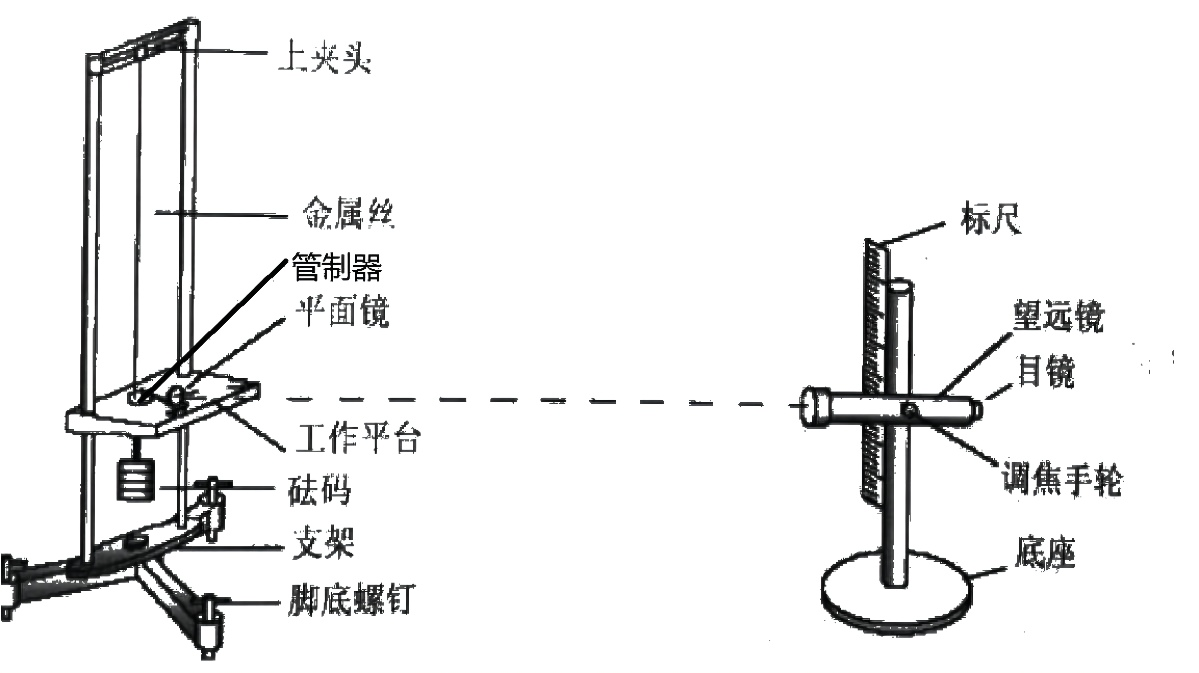
\includegraphics[width=\linewidth]{img/1.png}
        % \caption{示意图}
    \end{Figure}

    其中金属丝的长度约为$1m$,上端加紧在支架顶部。金属丝的下部连接了一个管制器,管制器连有一个法玛托盘,通过调节砝码盘上法码的数量可以调整受力,结合读数变化即可计算出杨氏模量的大小。

    \section{实验过程}

    \begin{itemize}
        \item 调节仪器:保持支架、工作平台水平;调整平台上下位置,与管制器顶部齐平。
    \end{itemize}

\end{multicols}
\end{document}